\chapter{Unit 1B}

\section{Fictitious Forces and Apparent Weight}
\subsection{Fictitious Forces}
\red{Fictitious forces} are also called \red{apparent forces} or \red{perceived forces}

\begin{redblock}
    \textbf{Explanation:} When the object is viewed from a \red{non-intertial F.O.R, we created fictitious force to explain the motion and behavior}
\end{redblock}

The \red{fictitious forces} will always act in the direction opposite to the direction of acceleration of 
the frame of reference.\\

\begin{cyanblock}
    The magnitude of each fictitious force can be calculated by:
    \[
        F_{fict} = m|\vec{a_{F.O.R}}|
    \]
\end{cyanblock}

Perceived acceleration could be represented by \red{$\vec{a_{per}}$}

\begin{redblock}
    \textbf{Note: } The object's actual acceleration would be measured relative to an inertia FOR
\end{redblock}

\subsection{Apparent Weight}
Technically, this would be the sum of the \red{normal force} and the force of \red{friction} that a surface exerts 
on an object. 

\subsection{Some of the formulas}
\[
    \sum \vec{F} = m\vec{a_{per}}
\]

\section{Lecture 2.5}
\subsection{Uniform Circular Motion}
\begin{redblock}
    \textbf{Direction}: The velocity of an object at any point along a circle has a direction that is 
    \red{tangential} to the circle
\end{redblock}

\columnratio{0.6, 0.4}
\begin{paracol}{2}
    \begin{leftcolumn}
        \textbf{Question:} If an object is attached to a string, swung in a circular motion and then the string is released,
        which of the five paths shown here will the object take?\\
        \red{ANS: Path 2}
    \end{leftcolumn}

    \begin{rightcolumn}
        \begin{center}
            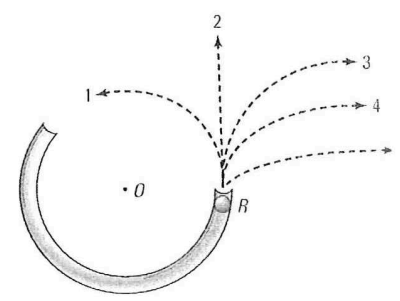
\includegraphics[width=0.3\textwidth]{graph/circularMotion.png}
        \end{center}
    \end{rightcolumn}
\end{paracol}

\subsection{Centripetal acceleration}
From the \red{Newton second law}, we understand that \red{An object will accelerate in the same 
direction as the net force}.

If the centripetal force is directed toward the centre of the circle, then what direction is the acceleration in?
\red{ANS: Toward the circle}

In other words, the acceleration will always \red{perpendicular} to the velocity of the object.

\subsection{Formulas}
\begin{cyanblock}
    Formula 1:
    \[
        \vec{a_{c}} = \frac{4 \pi ^2 R}{T^2}
    \]
    \[
        \vec{a_{c}} = 4\pi ^2 R f^2
    \]
    \[
        \vec{a_{c}} = \frac{V^2}{R}
    \]
    \begin{center}
        $\vec{a_{c}}$ is the acceleration of the object in $\frac{m}{s^2}$\\
        $R$ is the radius of the circular path that the object is moving around (in $m$)\\
        $T$ is the period of the object's motion \\
        $v$ is the speed of the object in (m/s)
    \end{center}
\end{cyanblock}

\begin{cyanblock}
    For clockwise:
    \begin{center}
        direction of acceleration = direction of velocity + 90 degree
    \end{center}
    else:
    \begin{center}
         direction of acceleration = direction of velocity - 90 degree
    \end{center}
\end{cyanblock}